From @FactoryBerlin, 10,000 followers were collected. Of these 10,000,
419 were selected as candidates. What made these users candidates was
that they were based in Berlin, and that they had a valid
friend:follower ratio. A valid friend:follower ratio means that there
was a disparity between the ratio of friends to followers of no
greater than 50\%. If there was a disparity greater than that, there
was an increased liklihood that the account was mass following users
in an attempt to grow their network (hoping that users will follow
back).

From those 419 candidates, a sample of 200 of their friends was
collected. Then, an analysis was performed to see if their ego-centric
friend network was composed of 2 or more sub-networks based in two
locales.  The subnetworks could not vary in size by more than 25\%. Of
those 419 candidates, only 56 were selected as potential Transnational
Entrpreneuers.

The first takeaway is: Transnational Entrepreneurs are exceedingly
rare. Of the 419 users that qualified for the initial analysis only
13.37\% were potentially Transnational Entrepreneurs.

From those 56 final Transnational Entrepreneur candidates, their
ego-centric network including their friends and followers (limit 200
for each) were extracted. Following this extraction, their friends and
followers were evaluated to make sure that they were not bots, and that
they were not spammers. This was checked in a number of ways, if they
were verified by Twitter, if they had a follower:friend ratio within
bounds of 75\%, if they had over 50 tweets, and if they were not just
retweeting the same information over 50\% of the time, they qualified.

From these Transnational Ego-Centric networks, we collected a total of
2412594 Tweets for analysis. Of these Tweets, we detected 263 counts
of transnational diffusion events. These events were sparsely related
to business, despite the individuals involved in them being focused on
business. This rate can increase or decrease depending on how broadly
we define two tweets to be related. More information follows.

From our approach, there are a few insurmountable, generalized
problems. The first major problem is that we were unable to tell
whether a Tweet or idea actually originated and was diffused by a
Transnational Entrepreneur. This is because are not directly measuring
the flow of information by probing the minds of individuals, and
instead observing their behavior on a network. For example, it is
wholly possible and likely that two or more users from two distinct
networks are listening to the same media source as the Transnational
Entrepreneur and receive their data from that source. To explain more
explicitly, imagine that all three individuals (the Transnational
Entrepreneur, the person from network A of the transnational, and the
persom from network B of the transnational) are all interested in
business. It is very possible that all three of them are following a
popular business leader on Twitter. In the case that the popular
business leader Tweets or disseminates knowledge that is interesting,
we may ``observe'' Transnational diffusion due to the ordering of the
Tweets within the Transnational's ego-centric network, whereas the
information actually originated from a third source. This of course
will always be a problem since we are not directly measuring what the
origin of information is, and are instead only assuming based upon our
percieved propagation of the data through the network.

The second major, generalized problem is that of parameterization.
When sifting through a data set of 2412594 tweets, it is not feasible,
for the purposes of this research, to go through them by hand. This
results in using algorithms and programs to identify and categorize
Tweets as being related. To do this, we used DB Scan, which does not
require us to know how many content clusters we will be expecting (in
contrast with K-Means and others). DB Scan is no silver bullet. One
has to manually run and re-run many tests against the data set to
determine the correct parameters for epsilon, and the minimum
samples. The epsilon value refers to the maximum distance between two
vectors for them to be considered part of the same cluster, and the
minimum samples refers to the minimum amount of vectors within epsilon
distance to constitute a cluster. The minimum sample size for a given
cluster in our project is obvious, three, that is the amount of tweets
that may constitute a transnational diffusion event. The harder value
to tweak is epsilon. Ultimately we decided on an epsilon value of 1.25
which minimizes the amount of false positives.

Note: One can also look at the distribution of data and attempt to
pick suitable epsilon values, but ultimately a human will have to
examine the output and verify that the program is behaving in
accordance with expectations.

Similarly with the DB Scan parameters, one has to also consider the
actual generation of vectors. Since we are using TF/IDF, we have to
tweak the minimum document frequency, maximum document frequency, and
possibly our stopword set and stemmer. This is an especially
challenging configuration due to the size of the documents on the
Twitter network (where words are also frequently
abbreviated). Ultimately we decided on using the NLTK stopword set, a
minimum document frequency of 0.0, a maximum document frequency of
0.80, and a porter stemmer to process and tokenize the text.

Lastly, when we plot our two data sets on the same graph, the delta
from a kurtosis of 3.0, and the amount of diffusion instances, we see
no significant relationship between the two variables. Therefore, the
null hypothesis is proven. There appears to be no moderation on
Transnational Diffusion activity as a product of the kurtosis in the
distribution of individuals in a given individuals network.
\begin{figure}[H]
  \centering
  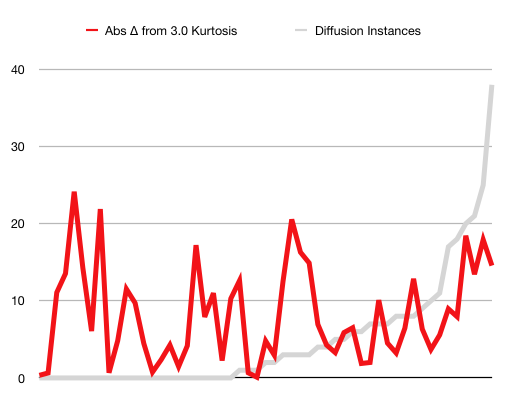
\includegraphics[width=1.0\textwidth]{delta_from_normal_distribution.png}
  \caption{The relationship between the amount of transnational diffusion instances, and the user's ego-centric network distribution kurtosis.}
\end{figure}

However, if we exclude all values below five diffusion instances, we
in fact see an inverse relationship of our hypothesis. There may in fact
be a relationship in the quantity and frequency of Transnational
Diffusion. Those with the most leptokurtic distributions may be those
who are most frequently involed in transnational diffusion. Looking at the
chart below, which omits transnationals with five or less diffusion instances
paints a quite different picture:
\begin{figure}[H]
  \centering
  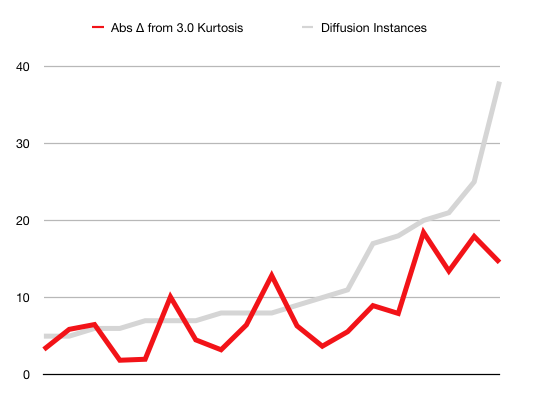
\includegraphics[width=1.0\textwidth]{trimmed_delta_from_normal_distribution.png}
  \caption{The relationship between the amount of transnational diffusion instances, and the user's ego-centric network distribution kurtosis, but only for users with 5 or more transnational diffusion events.}
\end{figure}
